% Chapter Template

\chapter{Analysis and Findings} % Main chapter title

\label{Chapter5} % Change X to a consecutive number; for referencing this chapter elsewhere, use \ref{ChapterX}

\section{Overview}

Having finalized our model, this chapter will focus on applying the model to the ICU patient population and subpopulations of it. We follow an iterative approach to our subgroup analysis. Based on the trend shown in a larger population, we hypothesize on potential splits in the population over which this trend may or may not persist. We then apply the model to these subpopulation and repeat the process. 

\section{General ICU Population}

Applying the model to our general ICU patient population we find that SF ratio is a significant predictor for patient mortality. Moreover, looking at figure \ref{fig:results_general} below, we find that below SF ratio of 180 the probability of mortality significantly increases, suggesting that 180 is an inflection point. 


\begin{figure}[H]
	\centering
	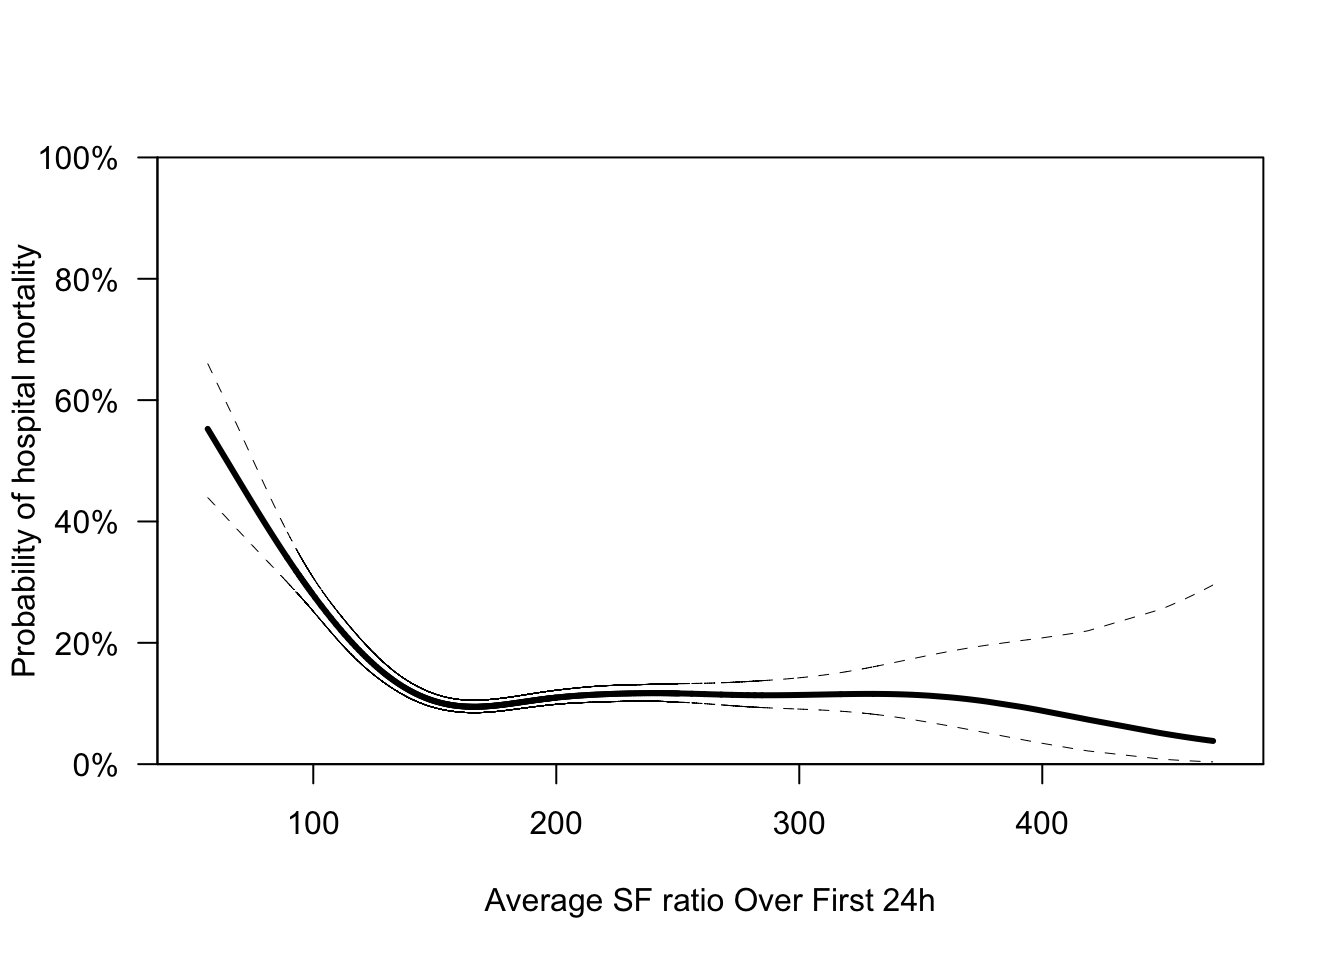
\includegraphics[width=0.9\textwidth]{figures/results_general-1.png}
	\caption{SF ratio vs Patient Mortality for General ICU Population} 
	\label{fig:results_general}
\end{figure}

\section{Subgroup Analyses}

\subsection{SF ratio as a Predictor in Patients with Different Oxygen Support}

\subsubsection{Hypothesis}
In an ICU setting, pulmonary support comes in two forms - invasive and non-invasive. Invasive mechanical ventilation involves the use of an instrument to penetrate the patients airway and serve as an artificial airway. On the other hand, non-invasive mechanical ventilation involves administering air with additional oxygen content through an external apparatus such as a mask \citep{davidson2016bts}. Invasive mechanical ventilation is considered a stronger form of support for more vulnerable patients as it performs parts of the breathing function for the patient. 

Since patients on invasive mechanical ventilation are more vulnerable than those on non-invasive mechanical ventilation, such patients should be at a higher risk of death at lower SF ratio compared to the general population. Our hypothesis is as follows: 

\textit{The trend between SF ratio and patient mortality is steeper in the patient population with invasive mechanical ventilation than in the general patient population. Similarly, the trend is less steep in the patient population with non-invasive mechanical ventilation than in the general patient population.
}


\subsubsection{Test and Observation}

We split the patient population depending on the type of oxygen support, and apply our model to each subpopulation. Subsequently, we plot each of the trends next to the trend in the general population. 

Figures \ref{fig:subgroupanalysis1-2} and \ref{fig:subgroupanalysis1-1} below confirm our hypothesis. A low SF ratio suggests a much higher risk of mortality in a patient on invasive mechanical ventilation than in a patient on non-invasive mechanical ventilation.  This suggests that SF ratio might be a specifically valuable predictor of patient outcome for patients on mechanical ventilation. 

\begin{figure}[H]
	\centering
	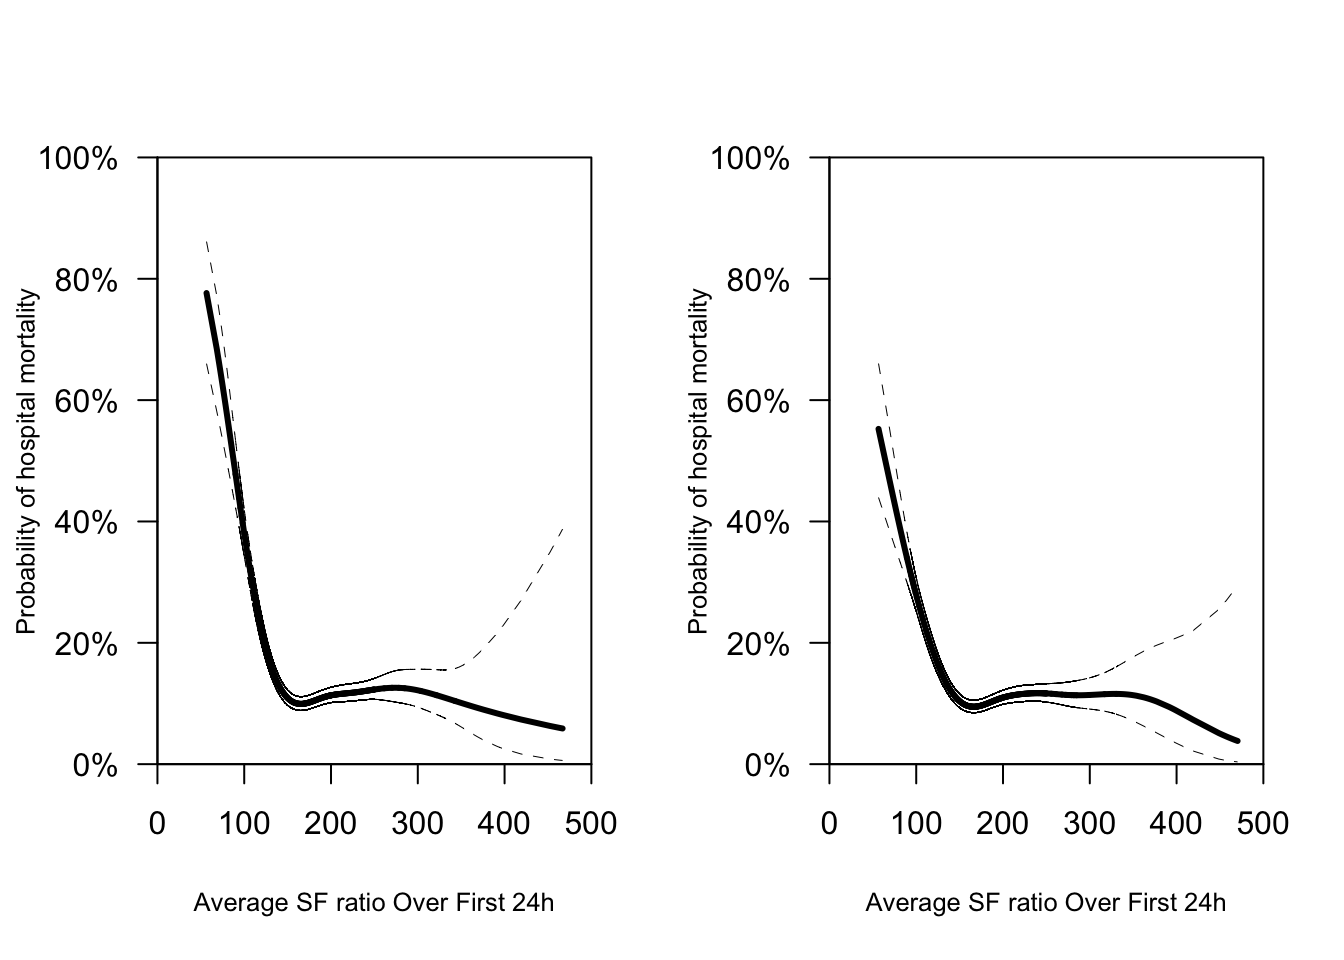
\includegraphics[width=0.9\textwidth]{figures/subgroupanalysis1-2.png}
	\caption{\textbf{Left:} Patients on Invasive Mechanical Ventilation \\ \textbf{Right:} General ICU Population}
	\label{fig:subgroupanalysis1-2}
\end{figure}


\begin{figure}[H]
	\centering
	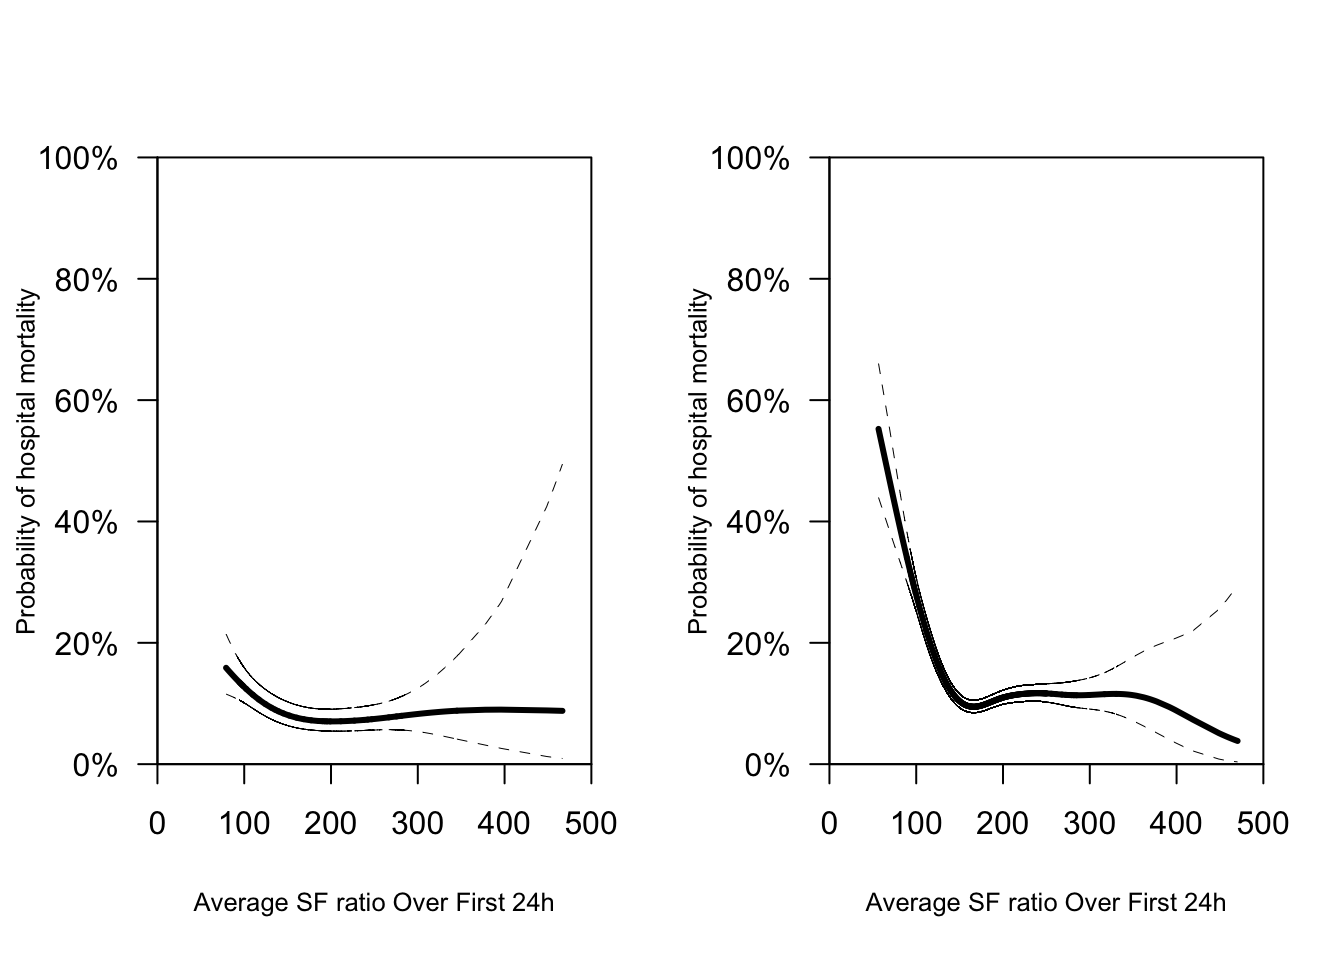
\includegraphics[width=0.9\textwidth]{figures/subgroupanalysis1-1.png}
	\caption{\textbf{Left:} Patients on Non-Invasive Mechanical Ventilation \\ \textbf{Right:} General ICU Population}
	\label{fig:subgroupanalysis1-1}
\end{figure}



\subsection{SF ratio as a Predictor in Patients with Different Levels of \Fi}

\subsubsection{Hypothesis}
A matter of debate in research pertaining to ICU care is the amount of \Fi to be administered to the patient with studies showing that both excess and shortage of inspired oxygen can be detrimental to certain ICU patients \citep{rachmale2012practice}. We explore whether the inflection point for our model remains constant for two patient subpopulations - those administered initial \Fi less than 50\% and those administered intial \Fi greater than 50\%. If the inflection point is the same for both groups, it could suggest a lower safety threshold of the SF ratio that can be targeted when deciding on level of \Fi to be administered. 

\subsubsection{Test and Observations}

We split the patient cohort into two groups - those administered initial \Fi less than 50\% and those administered intial \Fi greater than 50\%. Subsequently, we apply the model and plot the trends below. 

\begin{figure}[H]
	\centering
	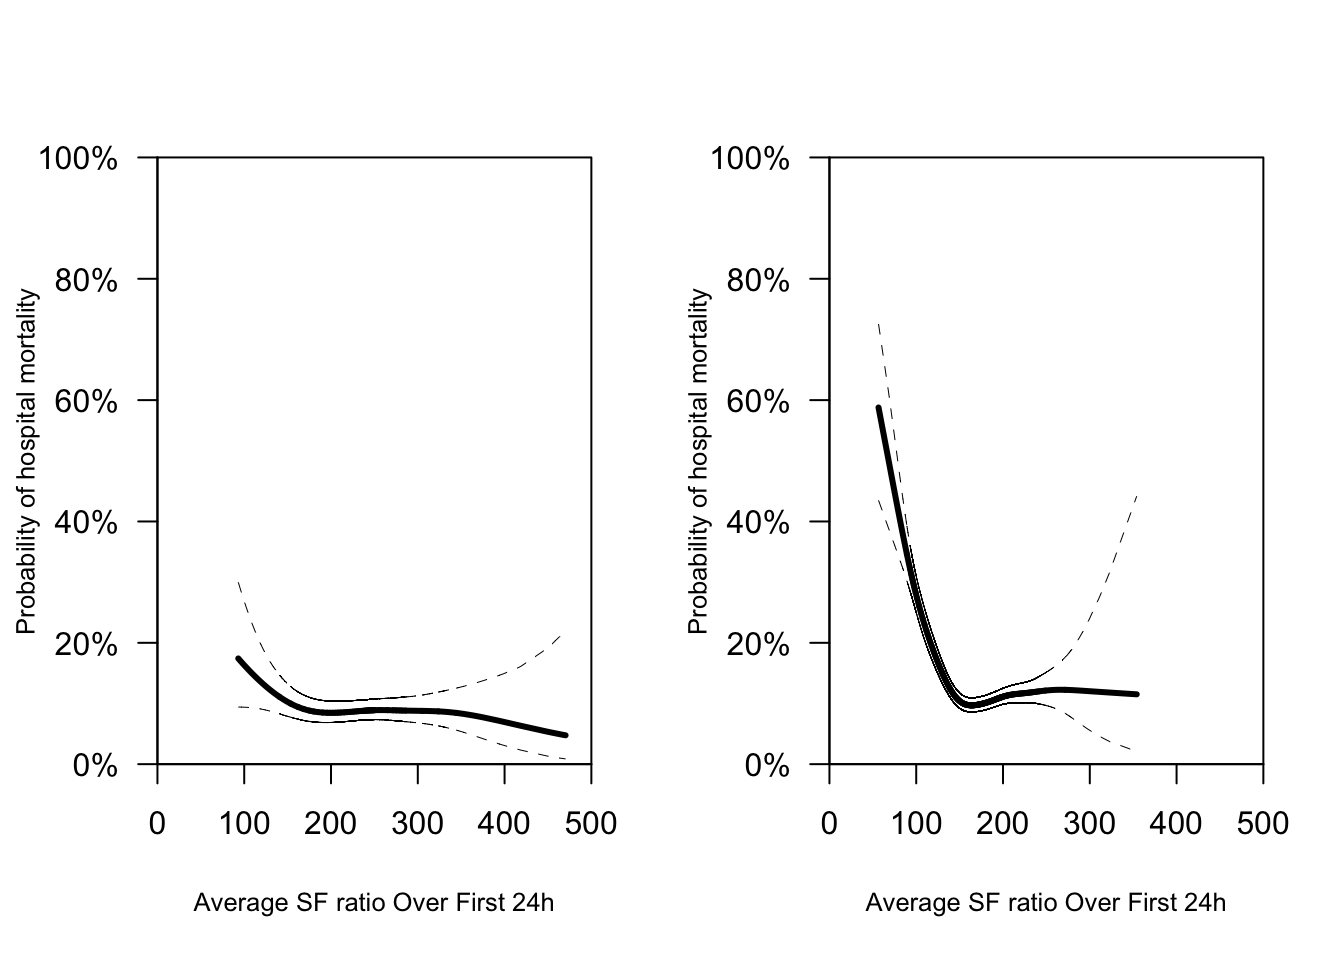
\includegraphics[width=0.9\textwidth]{figures/subgroupanalysis_fio2-1.png}
	\caption{\textbf{Left:} Patients with Initial \Fi > 50\\ \textbf{Right:} Patients with Initial \Fi < 50}
	\label{fig:subgroupanalysis_fio2-1}
\end{figure}

Figure \ref{fig:subgroupanalysis_fio2-1} suggests that there is no constant inflection point for patients with different levels of \Fi administered. For those with \Fi greater than 50\%, the inflection point is around 180, while for those with \Fi less than 50\%, the inflection point is around 150. Therefore, there does not seem to be a lower safety threshold for SF ratio that can be used to calibrate \Fi administration. 

However, this difference could suggest that the lower limit of safety is in terms of \Sp, not SF ratio. This would be interesting as there is disagreement in the target \Sp levels recommended by various national health organizations. For instance, the Thoracic Society of Australia and New Zealand recommends a target \Sp range of 92-96\%, while the British Thoracic Society recommends a target range of 94-98\%. Although beyond the scope of our research question, this provides potential for future research that could explore whether there indeed exists a \Sp safety threshold and further, whether that level is consistent across patient groups. 

